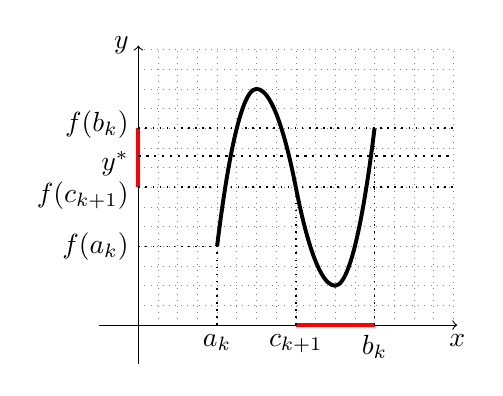
\begin{tikzpicture}
    % Рисуем сетку
    \draw[help lines, step=0.25, dotted]
    (-2,-2) grid (2,1.5);
    % Начало координат
    \draw[->, thin] (-2.5,-2) -- (2.05,-2)
    node[below] {$x$}; % Ox
    \draw[->, thin] (-2,-2.5) -- (-2,1.55)
    node[left] {$y$}; % Oy

    \draw[line width =.05cm](-1, -1) parabola bend (-0.5, 1) (0, -0.25);
    \draw[line width =.05cm](0, -0.25) parabola bend (0.5, -1.5) (1, 0.5);

    \draw[line width =.05cm, red] (1, -2) -- (0,-2);
    \draw[line width =.05cm, red] (-2, -0.25) -- (-2, 0.5);

    \draw[dotted, line width =.02cm] (-1, -2) -- (-1, -1);
    \draw[dotted, line width =.02cm] (0, -2) -- (0, -0.25);
    \draw[dotted, line width =.02cm] (1, -2) -- (1, 0.5);
    \draw[dotted, line width =.02cm] (-2, -1) -- (-1, -1);
    \draw[dotted, line width =.02cm] (-2, -0.25) -- (2, -0.25);
    \draw[dotted, line width =.02cm] (-2, 0.5) -- (2, 0.5);
    \draw[dotted, line width =.03cm] (-2, 0.15) -- (2, 0.15);

    \node[left] at (-2, 0.05) {$y^{*}$};
    \node[left] at (-2, 0.55) {$f(b_{k})$};
    \node[left] at (-2, -1) {$f(a_{k})$};
    \node[left] at (-2, -0.35) {$f(c_{k+1})$};
    \node[below] at (-1, -2) {$a_{k}$};
    \node[below] at (0, -2) {$c_{k+1}$};
    \node[below] at (1, -2) {$b_{k}$};
    \end{tikzpicture}